\section{3. Triển khai cấu hình thực tế mạng WLAN}

\textit{Phần này ghi chép lại toàn bộ quá trình thực hiện trong video đính kèm. Xuyên suốt quá trình cấu hình, mọi bước thiết lập đều có hình ảnh minh chứng xác thực từ thiết bị của nhóm.}

\subsection{3.1 Ghi nhận thông số ban đầu của Router}

Trước khi tiến hành cấu hình, nhóm thực hiện ghi nhận các thông số mạng hiện tại của Router bằng lệnh \texttt{ipconfig} trên máy tính client đang kết nối Wi-Fi với Router. Kết quả thu được như sau:

\begin{itemize}
    \item \textbf{Địa chỉ IPv4 của máy client:} \texttt{192.168.1.6}
    \item \textbf{Subnet Mask:} \texttt{255.255.255.0}
    \item \textbf{Default Gateway (địa chỉ IP của Router):} \texttt{192.168.1.1}
\end{itemize}

Từ Subnet Mask \texttt{255.255.255.0} (tương ứng \texttt{/24}), nhóm xác định được dải IP dự kiến sử dụng cho mạng nội bộ là:

\[
192.168.1.0/24 \quad \text{(từ } 192.168.1.1 \text{ đến } 192.168.1.254\text{)}
\]

trong đó địa chỉ \texttt{192.168.1.1} được Router sử dụng làm Default Gateway, các địa chỉ còn lại sẽ được cấp phát cho các thiết bị client thông qua DHCP.

\begin{figure}[H]
    \centering
    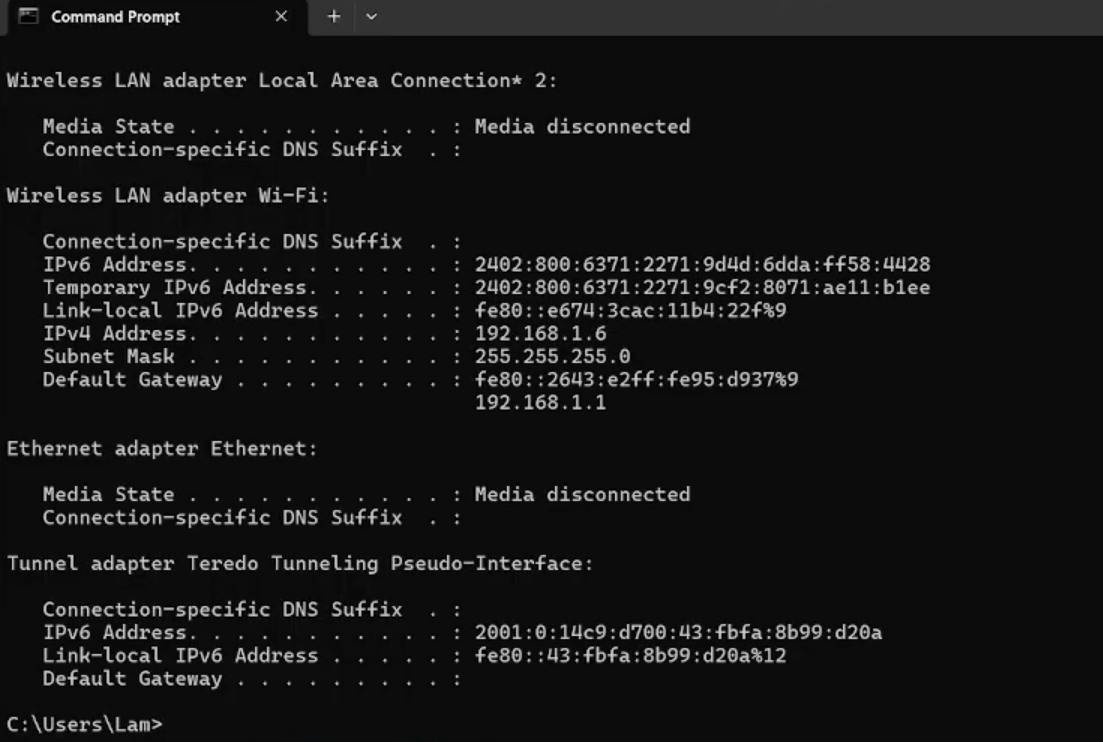
\includegraphics[width=0.8\textwidth]{image/ipconfig.png}
    \caption{Kết quả lệnh \texttt{ipconfig} hiển thị Default Gateway và địa chỉ IPv4 của máy client}
    \label{fig:ipconfig}
\end{figure}

Bên cạnh đó, thông tin tài khoản quản trị (Web Access) của Router được nhóm ghi nhận trực tiếp từ tem thông số kỹ thuật dán phía sau thiết bị, cụ thể như sau:

\begin{table}[H]
    \centering
    \caption{Thông số ban đầu của Router}
    \label{tab:router-info}
    \begin{tabular}{|l|l|}
        \hline
        \textbf{Thông số} & \textbf{Giá trị} \\
        \hline
        Model Router & H646GM-V (DASAN) \\
        \hline
        Default Gateway & 192.168.1.1 \\
        \hline
        Dải IP dự kiến & 192.168.1.0/24 \\
        \hline
        Web ID (tài khoản đăng nhập) & admin \\
        \hline
        Mật khẩu đăng nhập mặc định & DSNW2895d930 \\
        \hline
        SSID mặc định (2.4G/5G) & VIETTEL\_GPON\_95D930 \\
        \hline
    \end{tabular}
\end{table}

\begin{figure}[H]
    \centering
    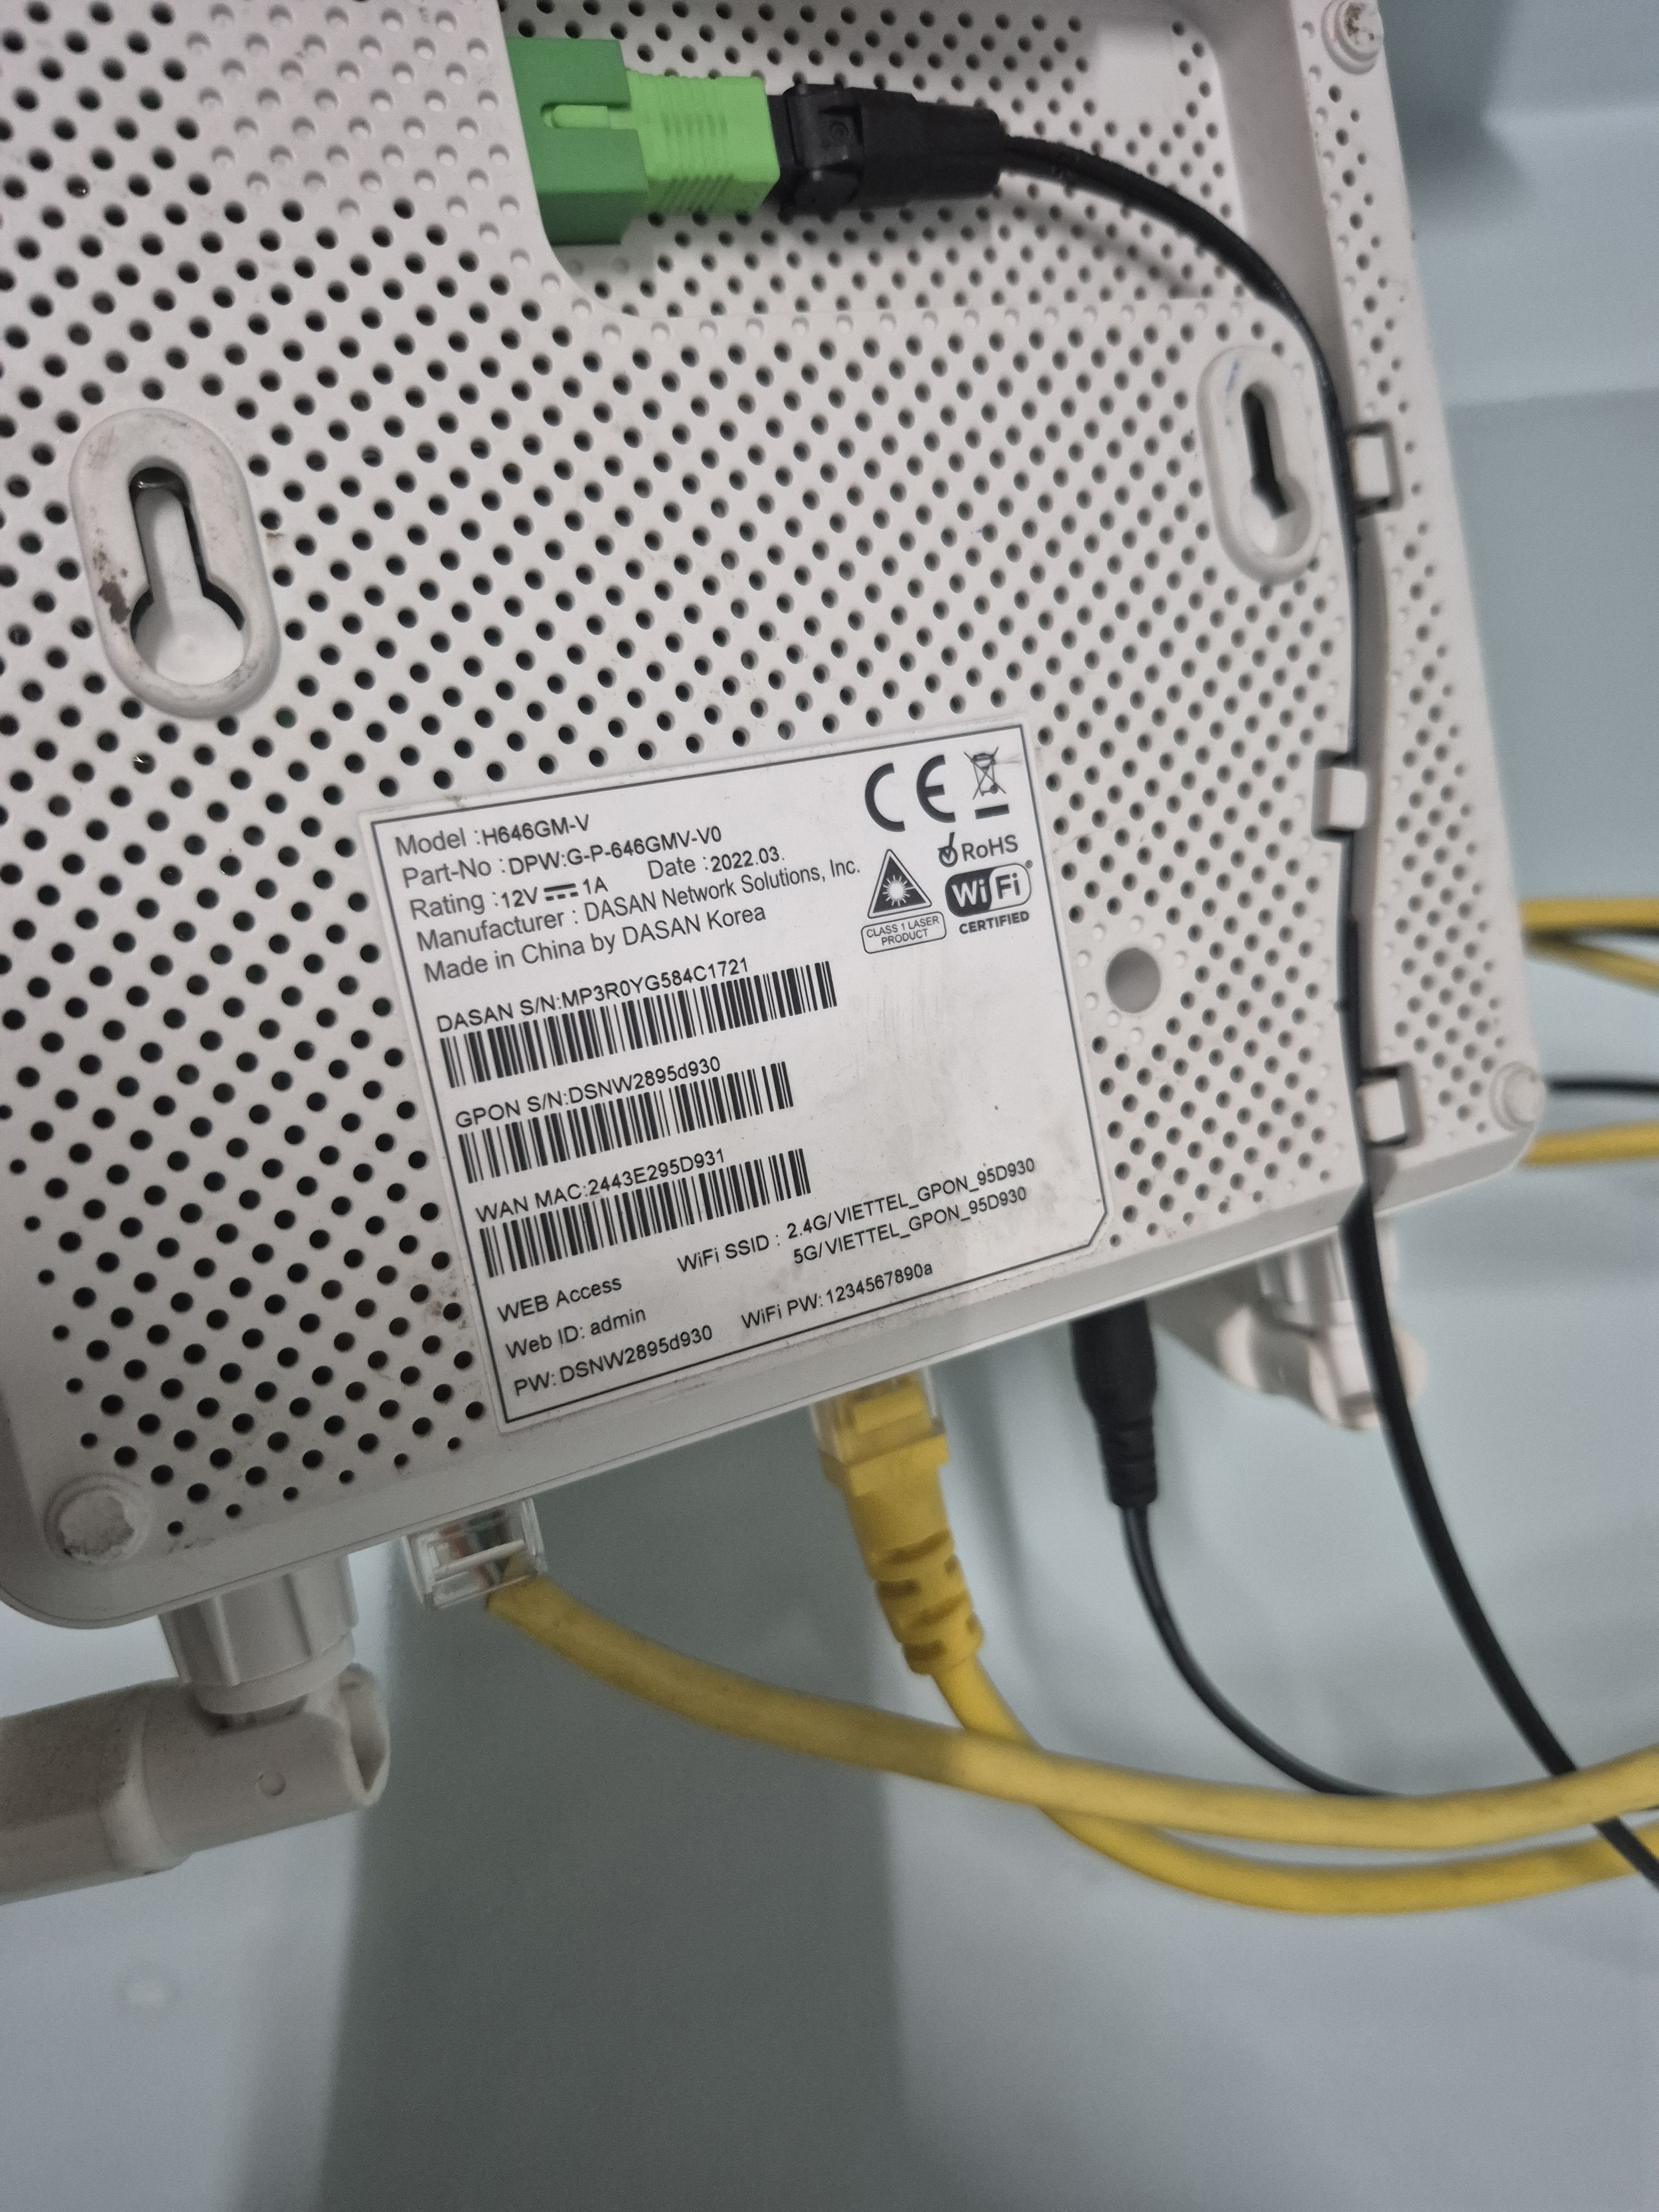
\includegraphics[width=0.7\textwidth]{image/tem-router.jpg}
    \caption{Tem thông số kỹ thuật mặt sau Router H646GM-V thể hiện Web ID, mật khẩu quản trị và SSID mặc định}
    \label{fig:tem-router}
\end{figure}

Các thông số này là cơ sở để nhóm thực hiện truy cập vào trang quản trị Router ở bước tiếp theo.

\subsection{3.2 Đăng nhập trang quản trị và thiết lập SSID}

Sau khi đã có đầy đủ thông số cần thiết, nhóm tiến hành đăng nhập vào trang quản trị của Router và cấu hình lại tên mạng (SSID) theo đúng quy chuẩn đặt tên của nhóm. Các bước thực hiện cụ thể như sau:

\begin{enumerate}
    \item \textbf{Truy cập trang quản trị:} Mở trình duyệt web trên máy client đang kết nối cùng mạng với Router, nhập địa chỉ Default Gateway đã ghi nhận ở mục 3.1 vào thanh địa chỉ:
    \[
    \texttt{http://192.168.1.1}
    \]

    \item \textbf{Đăng nhập hệ thống:} Tại giao diện đăng nhập của Viettel hiển thị tên model Router \texttt{H646GM-V}, nhóm nhập tài khoản và mật khẩu quản trị đã ghi nhận:
    \begin{itemize}
        \item Tên đăng nhập: \texttt{admin}
        \item Mật khẩu: \texttt{DSNW2895d930}
    \end{itemize}
    sau đó nhấn nút \textbf{Login} để truy cập vào trang quản trị.

    \begin{figure}[H]
        \centering
        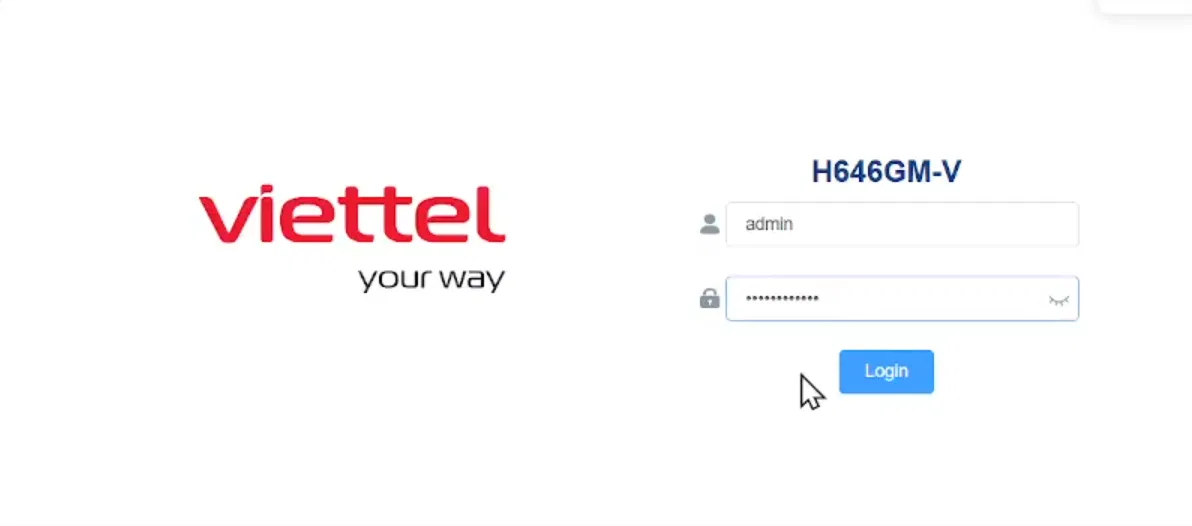
\includegraphics[width=0.7\textwidth]{image/login-router.png}
        \caption{Giao diện đăng nhập trang quản trị Router Viettel H646GM-V}
        \label{fig:login-router}
    \end{figure}

    \item \textbf{Truy cập mục cấu hình Wi-Fi:} Từ giao diện quản trị, nhóm chọn mục \textbf{Easy Setup} để truy cập đến phần thiết lập thông số Wi-Fi 2.4GHz (\textit{WiFi 2.4GHz Settings}).

    \item \textbf{Thiết lập SSID theo chuẩn nhóm:} Tại \textbf{Network Name}, nhóm tiến hành đổi tên mạng từ giá trị mặc định sang tên theo đúng định dạng quy ước của đồ án:
    \[
    \texttt{25CLC10-N07}
    \]
    Giữ nguyên loại xác thực \textbf{Authentication Type} là \texttt{WPA2-PSK} và mật khẩu Wi-Fi (\textit{Pre-Shared Key}) là \texttt{1234567890a}. Do tính năng \textbf{Band Steering} đang ở trạng thái \texttt{Enabled}, băng tần 2.4GHz và 5GHz sẽ tự động sử dụng chung một tên SSID.

    \begin{figure}[H]
        \centering
        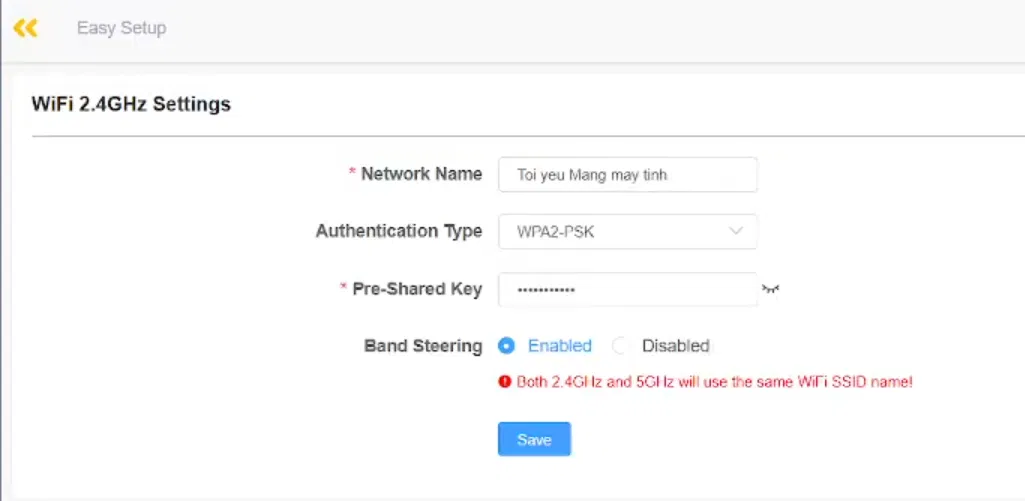
\includegraphics[width=0.7\textwidth]{image/ssid-truoc-doi.png}
        \caption{Giao diện \textit{Easy Setup} -- WiFi 2.4GHz Settings trước khi đổi tên mạng (SSID mặc định)}
        \label{fig:ssid-truoc}
    \end{figure}

    \item \textbf{Lưu cấu hình:} Nhấn nút \textbf{Save} để hoàn tất việc đổi tên mạng. Sau khi lưu thành công, trang quản trị hiển thị lại tên mạng mới là \texttt{25CLC10-N07}, xác nhận việc thiết lập SSID đã được áp dụng đúng theo chuẩn định dạng của nhóm.

    \begin{figure}[H]
        \centering
        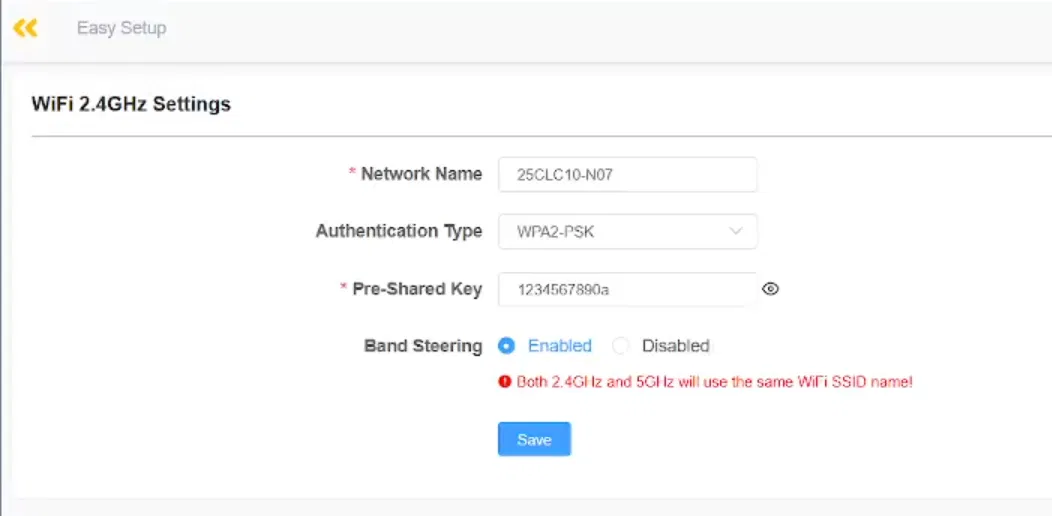
\includegraphics[width=0.7\textwidth]{image/ssid-sau-doi.png}
        \caption{Giao diện \textit{Easy Setup} sau khi cập nhật tên mạng theo chuẩn định dạng của nhóm}
        \label{fig:ssid-sau}
    \end{figure}
\end{enumerate}

\subsection{3.3 Cấu hình thiết bị đầu cuối}
Quá trình kết nối từng loại thiết bị vô mạng kèm hình ảnh minh chứng kiểm tra thành công:

\subsection{3.4 Triển khai Mạng Ad-hoc}
\textit{Chú ý: Do thiết bị thực tế của nhóm đang chạy hệ điều hành [Tên HĐH] không còn hỗ trợ tạo Ad-hoc trực tiếp, nhóm đã thực hiện cấu hình mạng Ad-hoc trên máy ảo.}